\chapter{Background}

This chapter provides a description of basic concepts and theory used in this thesis.
The first section presents basic concepts of graph theory.
Graph theory is largely used throughout the literature of compiler construction and compilation techniques.
Second is an overview of the LLVM compiler infrastructure.

\section{Basic Concepts of Graph Theory}

In graph theory, a \textit{graph} is an ordered pair $G = (V,E)$ comprising a vertex-set $V$ and an edge-set $E$, where $E \subset V\times V$.
For any two vertices $u,v\in V$, vertices $u$ and $v$ are said to be adjacent vertices if and only if $\{u,v\}\in E$.
A graph is directed when each edge is represented by an ordered pair, in which case a directed edge $(u,v)\in E$ contains a source vertex $u$ and a target vertex $v$.

A \textit{path} in a graph is a sequence of edges that compose a chain of adjacent vertices.
An undirected graph is connected if there is a path between any two vertices of the graph.
If an undirected graph is called a \textit{tree} if and only if it is both connected and acyclic.
For any graph $G = (V,E)$, if a subgraph $H$ of $G$ is a tree and contains all vertices in $V$, then $H$ is called a \textit{spanning tree}.

\subsection{Maximum Spanning Tree}

For weighted graphs, i.e., graphs for which their edges have weights associated with them, a minimum or maximum spanning tree is a spanning tree for which
the sum of the weights that comprise the spanning tree is minimum or maximum, respectively.
The problem of finding the maximum (or minimum) spanning tree is a polynomial-time function problem~\citep{kruskal56,bazlamacci01}.

There are several efficient algorithms for solving the problem of finding a maximum (or minimum) spanning tree in a greedy manner\footnote{The problem of finding a maximum spanning tree can be solved by the same solution that finds a minimum spanning tree just by negating the edge weights.} \citep{bazlamacci01}.
A well-known efficient algorithm is Kruskal's algorithm~\citep{kruskal56}.
Kruskal's algorithm works in a greedy manner with a single pass over the edges sorted in increasing order.
It starts with a forest of singleton graphs, i.e., a set of disjoint trees where each tree comprises a single vertex.
The algorithm evaluates all edges in increasing order, joining disconnected trees into larger trees.
In the end, there is a single tree connecting all vertices of the graph with minimum total weight.

\begin{lstlisting}[caption={Kruskal's algorithm for finding a minimum spanning tree}, label={lst:kruskalMST}, float]
// Input: Undirected Graph
// Output: Minimum Spanning Tree
kruskalMST(G) {
  MST = set{}
  UF = unionFindSet()
  for v in G.vertices():
    UF.makeSet(v)
  sortedEdges = sortByWeight(G.edges(), order=increasing)
  for {u,v} in sortedEdges:
    //if u and v belong to distinct trees,
    //join the trees with the edge {u,v}
    if UF.find(u) != UF.find(v):
       MST = MST union set{ {u,v} }
       UF.@union@(u,v)
  return MST
}
\end{lstlisting}

\lstlistingname~\ref{lst:kruskalMST} shows an implementation of Kruskal's algorithm using an efficient data structure called the union-find data structure~\citep{hopcroft73,tarjan75}.
The union-find data structure provides three near-constant-time operations, namely \verb|makeSet|, \verb|find| and \verb|union|.
It allows the Kruskal's algorithm to efficiently keep track of the trees contained in the forest and efficiently join two disconnected trees into a single larger tree~\citep{galil91}.

\section{LLVM Compiler Infrastructure}

LLVM was originally proposed as a \textit{Low-Level Virtual Machine}\footnote{Although LLVM was initially an acronym for Low-Level Virtual Machine, it is now a brand that applies to the whole LLVM umbrella project.}, extending previous work on virtual instruction set architectures~\citep{adve03,lattner04}.
Since then, LLVM has evolved into an umbrella project that comprises a collection of modular and reusable compiler and toolchain technologies.
The main components under the LLVM umbrella is the LLVM intermediate representation (IR) and the LLVM \textit{Core} libraries.

The LLVM compiler infrastructure implements the classical \textit{three-phase compiler} infrastructure, which consists of a frontend, an optimiser, and a backend, as depicted in Figure~\ref{fig:3-phase-compiler}.
The frontend is responsible for parsing, validating and diagnosing errors in the source code.
This parsed source code is then translated into an intermediate representation, which is the LLVM IR in this case.
The optimiser is responsible for doing a broad variety of transformations, that are usually independent of language and target machine, to improve the code's performance.
%The front end parses source code, checking it for errors, and builds a language-specific Abstract Syntax Tree (AST) to represent the input code. The AST is optionally converted to a new representation for optimization, and the optimizer and back end are run on the code.
%The optimizer is responsible for doing a broad variety of transformations to try to improve the code's running time, such as eliminating redundant computations, and is usually more or less independent of language and target.
The backend, also known as the code generator, then translates the code from the intermediate representation onto the target instruction set.
It is common for the backend to also perform some low-level optimisations that take advantage of unusual features of the supported architecture.
%Common parts of a compiler backend include instruction selection, register allocation, and instruction scheduling.

\begin{figure}[h]
  \centering
  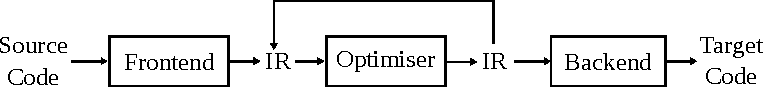
\includegraphics[scale=0.9]{figs/3-phase-compiler.pdf}
  \caption{Overview of the three-phase compiler infrastructure.}
  \label{fig:3-phase-compiler}
\end{figure}

%This IR is optionally fed through a series of analysis and optimization passes which improve the code, then is sent into a code generator to produce native machine code, as shown in Figure 11.3.
%This is a very straightforward implementation of the three-phase design, but this simple description glosses over some of the power and flexibility that the LLVM architecture derives from LLVM IR.

%The most important aspect of its design is the LLVM Intermediate Representation (IR), which is the form it uses to represent code in the compiler.
%LLVM IR is designed to host mid-level analyses and transformations that you find in the optimizer section of a compiler.
%It was designed with many specific goals in mind, including supporting lightweight runtime optimizations, interprocedural optimizations, whole program analysis, and aggressive restructuring transformations, etc.

%Like a real RISC instruction set, it supports linear sequences of simple instructions like add, subtract, compare, and branch.

\subsection{LLVM Virtual Instruction Set}

LLVM IR is a low-level RISC-like virtual instruction set.
It differs from other intermediate representations (e.g. GCC's GENERICS or the most recent GCC's GIMPLE) as it is defined as a first class language with well-defined semantics.
Beyond being implemented as a language, LLVM IR is actually defined in three isomorphic forms: the textual format above, an in-memory data structure inspected and modified by optimizations themselves, and an efficient and dense on-disk binary \textit{bitcode} format.
%The LLVM Project also provides tools to convert the on-disk format from text to binary: llvm-as assembles the textual .ll file into a .bc file containing the bitcode goop and llvm-dis turns a .bc file into a .ll file.

Unlike most RISC instruction sets, LLVM is strongly typed with a simple language-independent type system.
LLVM's type system can be used to implement data types and operations from high-level languages exposing their implementation behaviour to all stages of optimisation.
This type system includes the type information used by sophisticated techniques, such as algorithms for pointer analysis, dependence analysis, and data transformations.
LLVM also offers instructions for performing type conversions and low-level address arithmetic while preserving type information.
Furthermore, LLVM IR also differs from RISC instruction sets as some details of the machine are abstracted away.
For example, the calling convention is abstracted through call and ret instructions and explicit arguments.
Another significant difference from machine code is that the LLVM IR has an infinite set of virtual registers (which are named with a \% character), insted of having just a fixed set of named registers.

The LLVM type system is considered one of the most important features of its intermediate representation, as it enables several optimisations to be performed directly on the IR, without having to do extra analyses on the side before the transformation.
The main first class types supported are: single value types, aggregate types, and labels.
Single value types consist of integers of arbitrary bit width (e.g.\lstinline[language=llvm,style=nasm]{i32} denotes a 32-bit integer), floating-point of commonly used width (e.g.\lstinline[language=llvm,style=nasm]{half},\lstinline[language=llvm,style=nasm]{float},\lstinline[language=llvm,style=nasm]{double}, and\lstinline[language=llvm,style=nasm]{fp128}), pointers (e.g.\lstinline[language=llvm,style=nasm]{i32*}) and vector types.
Vectors are used when multiple primitive data are operated in parallel using a single instruction (SIMD).
A vector type is represented by a the number of elements and an underlying primitive data type, e.g.\lstinline[language=llvm,style=nasm]{<4 x i32>} is a vector of four 32-bit integer values.
Aggregated types consist of arrays and structures.
Vectors are not considered to be aggregate types.

In addition to type information, LLVM IR also provides other high-level information that are useful for effectively performing several code analysis and transformations.
This includes explicit control flow graphs (CFG)~\citep{allen70} and an explicit dataflow representation, by means of the infinite register set in \textit{static single assignment} (SSA) form~\citep{alpern88,cytron89,cytron91}.

A control flow graph (CFG) is a directed graph in which the nodes represent basic blocks and the edges represent control flow paths, i.e. edges represent transfers of control (jumps) between basic blocks.
A basic block is a straight-line sequence of instructions having only one entry point, i.e. the first instruction to be executed in the basic block, and only one exit point, i.e. the last instruction executed~\citep{allen70,cytron91}.
Figure~\ref{fig:cfg-odd_inc} shows an example of a CFG constructed from the code in Listing~\ref{lst:ex:odd_inc}.

An IR is in SSA form if and only if each virtual register is assigned exactly once and every use of registers occur after their definition.
The primary advantage of using the SSA form is that it simultaneously simplifies and improves several compiler optimisations and analysis~\citep{alpern88,cytron91}.
Most of the industrial-strength compilers for imperative programming language rely heavily on the SSA form.

\begin{lstlisting}[language=llvm,style=nasm,caption={An illustrative example of a function in textual LLVM IR. This function returns the argument incremented by one if it is even or by two if it is an odd integer.}, label={lst:ex:odd_inc}]
define i32 @odd_inc(i32 %arg) {
entry:
  %rem = srem i32 %arg, 2
  %cmp = icmp eq i32 %rem, 0
  br i1 %cmp, label %if.then, label %if.else
if.then:
  %add.1 = add i32 %arg, 1
  br label %if.end
if.else:
  %add.2 = add i32 %arg, 2
  br label %if.end
if.end:
  %ans = phi i32 [ %add.1, %if.then ], [ %add.2, %if.else ] [!\label{lst:odd_inc:phi}!]
  ret i32 %ans
}
\end{lstlisting}

Listing~\ref{lst:ex:odd_inc} shows an example of a function written using textual LLVM IR.
Names starting with the @ character have a global scope, while names starting with \% have a local scope.
As stated previously, LLVM IR is strongly typed, which means that every virtual register is attributed a specific type (e.g.\lstinline[language=llvm,style=nasm]{i32 %arg} is of type\lstinline[language=llvm,style=nasm]{i32}, namely a 32-bit integer) as well as every operation (e.g.\lstinline[language=llvm,style=nasm]{add i32} expects all operands of type\lstinline[language=llvm,style=nasm]{i32}).
Instructions use the three address format, which refers to the use of three operands by most of the instructions.
However, instructions with fewer or more operands may occur, e.g. the\lstinline[language=llvm,style=nasm]{ret} instruction have fewer operands, while the\lstinline[language=llvm,style=nasm]{phi} and the\lstinline[language=llvm,style=nasm]{call} instructions may have more than three operands.

Furthermore, the SSA form requires a special assignment statements called the $\phi$-function (see line \ref{lst:odd_inc:phi} of Listing~\ref{lst:ex:odd_inc}).
The $\phi$-function receives as argument a list of virtual registers from different  control flow predecessors of the point where the $\phi$-function occurs.
The control flow predecessors of each point in the CFG are listed in some arbitrary fixed order, and the $i$-th operand of $\phi$-function is associated with the $i$-th predecessor.
If control reaches the $\phi$-function from its $i$-th predecessor, then the value of the $i$-th operand is attributed in the assignment.
Each execution of a $\phi$-function uses only one of the operands, but which one depends on the flow of control just before the $\phi$-function.

\begin{figure}[h]
  \centering
  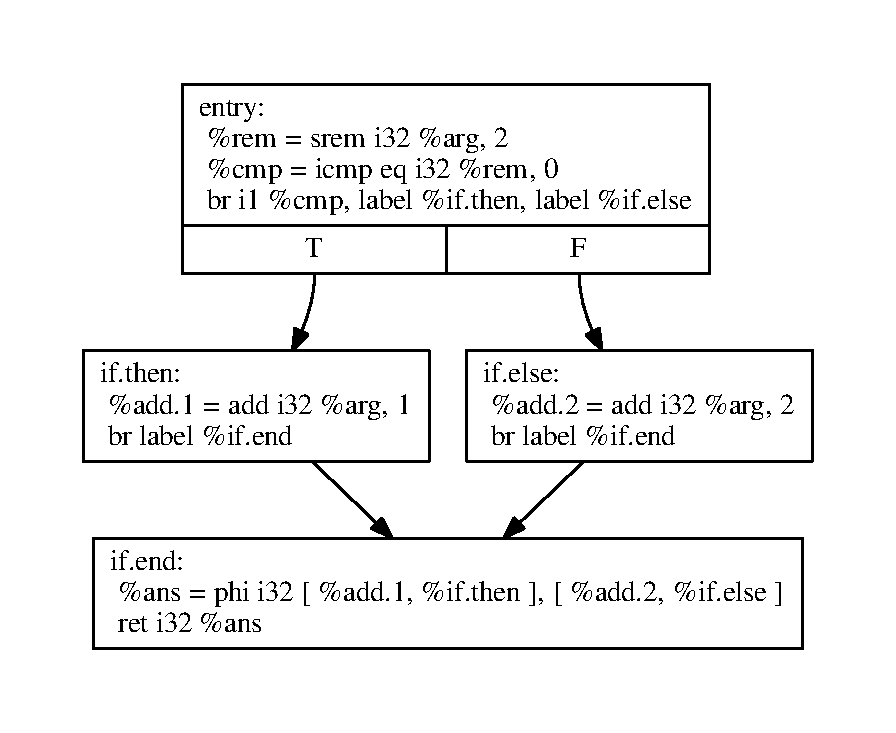
\includegraphics[scale=0.7]{figs/cfg-odd_inc.pdf}
  \caption{Control flow graph of the\lstinline[language=llvm,style=nasm]{odd_inc} function (see Listing~\ref{lst:ex:odd_inc}).}
  \label{fig:cfg-odd_inc}
\end{figure}

In addition to virtual registers, LLVM also allows for stack allocated local variables.
These are created by allocating data on the stack frame of the currently executing function.
Data from the stack frame can be manipulated by using explicit memory access operations.
Figure~\ref{lst:ex:odd_inc_stack} shows an implementation of the\lstinline[language=llvm,style=nasm]{odd_inc} function using data allocated on the stack frame.
This implementation avoids using the $\phi$-function by keeping the answer on the stack.
This is the preferred way of generating LLVM code by most frontends, as it simplifies the frontend's own implementation without incurring any serious detriment to the generated code.

LLVM provides an optimisation pass for promoting memory references to be register references (called \texttt{-mem2reg}).
It promotes alloca instructions which only have loads and stores as uses.
An alloca is transformed by using dominator frontiers to place phi nodes, then traversing the function in depth-first order to rewrite loads and stores as appropriate.

\begin{lstlisting}[language=llvm,style=nasm,caption={An example of the odd\_inc function implemented using data allocated on the stack frame.}, label={lst:ex:odd_inc_stack}]
define i32 @odd_inc_stack(i32 %arg) {
entry:
  %addr = alloca i32
  %rem = srem i32 %arg, 2
  %cmp = icmp eq i32 %rem, 0
  br i1 %cmp, label %if.then, label %if.else
if.then:
  %add.1 = add i32 %arg, 1
  store i32 %add.1, i32* %addr
  br label %if.end
if.else:
  %add.2 = add i32 %arg, 2
  store i32 %add.2, i32* %addr
  br label %if.end
if.end:
  %ans = load i32, i32* %addr
  ret i32 %ans
}
\end{lstlisting}

%\textbf{Another difference between LLVM and GCC:}

%In particular, LLVM IR is both well specified and the only interface to the optimizer.
%This property means that all you need to know to write a front end for LLVM is what LLVM IR is, how it works, and the invariants it expects.
%Since LLVM IR has a first-class textual form, it is both possible and reasonable to build a front end that outputs LLVM IR as text, then uses Unix pipes to send it through the optimizer sequence and code generator of your choice.

%It might be surprising, but this is actually a pretty novel property to LLVM and one of the major reasons for its success in a broad range of different applications.
%Even the widely successful and relatively well-architected GCC compiler does not have this property: its GIMPLE mid-level representation is not a self-contained representation.
%As a simple example, when the GCC code generator goes to emit DWARF debug information, it reaches back and walks the source level "tree" form.
%GIMPLE itself uses a "tuple" representation for the operations in the code, but (at least as of GCC 4.5) still represents operands as references back to the source level tree form.

%The implications of this are that front-end authors need to know and produce GCC's tree data structures as well as GIMPLE to write a GCC front end.
%The GCC back end has similar problems, so they also need to know bits and pieces of how the RTL back end works as well.
%Finally, GCC doesn't have a way to dump out "everything representing my code", or a way to read and write GIMPLE (and the related data structures that form the representation of the code) in text form. The result is that it is relatively hard to experiment with GCC, and therefore it has relatively few front ends.

\subsection{Analysis and Transformation Passes}

The LLVM optimiser offers several passes in order to provide analysis and transformation capabilities.
These passes are written using the LLVM Core libraries and they are as loosely coupled as possible.
In other words, each pass is either a stand-alone pass or it explicitly declares its dependencies among other passes, in the case where it depend on some other analysis.
A pass can also specify the analysis passes that will be invalidated by its execution.

The LLVM Core libraries provide both analysis and transformation passes for different levels of the input program.
These levels, in hierarchical order, are: module, call-graph SCC, function, loop, single-entry single-exit region (or only region for short), and basic block.
A module is an entire \textit{translation unit} (e.g., a C/C++ file with all its headers included).
A pass level only allows modification inside the component in focus.
For example: while a module-level pass can operate on the entire module at once,
a function-level pass prohibits any modification on the module-level (or other functions).

\begin{figure}[h]
  \centering
  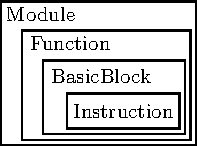
\includegraphics[scale=1]{figs/llvm-containers.pdf}
  \caption{The hierarchical levels in an LLVM input program. A call-graph SCC is a particular pattern amongst the functions in a module.
Similarly, a loop and a region are particular patterns on the CFG of a function.}
  \label{fig:llvm-containers}
\end{figure}

%\begin{description}
%\item[Module Pass:] This pass level allows the entire module to be analysed at once.
%\item[Function Pass:] This pass operates on each individual function contained in the module being processed.
%There is no particular order in which the functions will be considered.
%This pass level prohibits any modification on the module-level (or other functions).
%\item[Basic Block Pass:] This pass level considers one basic block at a time.
%\end{description}

The LLVM Pass Manager is responsible for scheduling the passes and make sure that the interactions among the passes are correctly fulfilled.
For that purpose, when given a series of passes to execute, the Pass Manager uses the explicit dependency information to satisfy these dependencies and optimise the execution of passes.
The Pass Manager aims at avoiding to repeat the execution of analysis passes.
It keeps track of which analyses are already available, which are invalidated, and which analyses are pending.
It also tracks the lifetimes of the analysis results and frees memory of the analysis results, when appropriate, managing memory usage.
%The Pass Manager pipelines the passes together to get a better memory and cache usage, improving the overall cache behaviour of the compiler.
For example, when performing a series of function-level passes, it executes all these passes in only one function, before moving to the next function, in order to improve the overall cache behaviour of the compiler.

Notice however, that the Pass Manager executes the transformation passes in the exact same order as they were requested, as changing this order may result in a different code.
Deciding on the best order to execute the transformation passes is a well known problem called the phase-ordering problem~\citep{touati06,kulkarni12,jantz14}.
The phase-odering problem is not addressed by the Pass Manager.

\section{{\IterComp} and its Optimisation-Space Exploration}

In this section we present the basic concepts of {\itercomp} and discuss some of the early work on this research topic.
We also consider some of the challenges on reducing its compilation time and present recent work that addresses these challenges.

{\Itercomp} is a well known compilation technique that searches the optimisation space in order to find the best optimisation for a particular program.
{\Itercomp} has the ability to adapt to new platforms, program and workload while still having a systematic and simple optimisation process.
It works by repeatedly evaluating a large number of compiler optimisations, by means of an execution-driven search, until the best optimisation is found for a particular program~\citep{kisuki99,fursin07,chen10}.
%The main challenge concerning {\itercomp} is the need for efficiently exploring such a large optimisation space~\citep{fursin07,cavazos07,zhou12}.

Figure~\ref{fig:itercomp-diagram} shows an overview of the architecture necessary for performing {\itercomp}.
After executing an optimised version of the program, profiling data is provided as a feed-back to the iterative search.
This profiling data can be as simple as the program's execution time, or more complex, including hardware performance counters for cache behaviour, measurements of energy consumption, etc.
The evaluator is able to use the feed-back in order to rank the optimisations and select the best one.
The optimisation generator can be a fixed sequence of optimisations or a dynamic mechanism for suggesting the next optimisation.

\begin{figure}[htb]
    \centering
    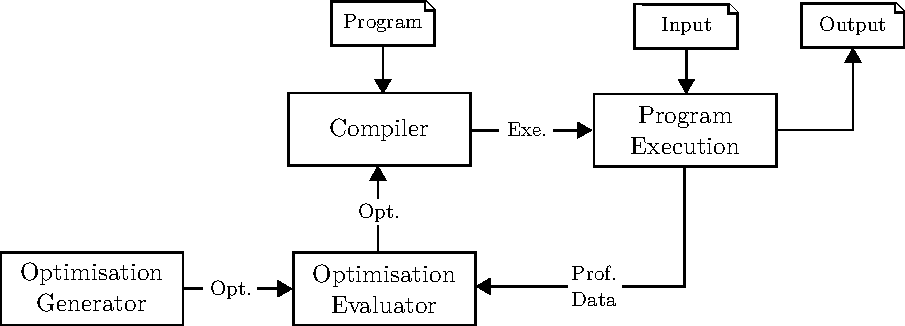
\includegraphics[width=\linewidth]{figs/itercomp-diagram}
    \caption{A simplified overview of the architecture of an iterative compiler.}
    \label{fig:itercomp-diagram}
\end{figure}

Early work on {\itercomp} demonstrated its use for determining simultaneously optimal tile sizes and unroll factors for any given loop nest~\cite{kisuki00,knijnenburg04}.
These two transformations are highly interdependent with a very irregular optimisation space, as both of them affect, in different ways, cache behaviour and instruction-level parallelism.
Because of their close interaction, with non-trivial trade-offs, designing a static cost model, that enables the compiler to automatically select the best configuration, is a very laborious and impractical task.
\cite{kisuki00} propose the use of {\itercomp} to address this problem, where it is able to outperform several static techniques.
However, its success comes at the cost of a significant increase in compilation time, which involves several runs of the program for the execution-driven search.

Despite the high cost of compilation time, there are scenarios where this approach is highly attractive due to high-performance requirements, such as embedded systems and library codes.
Moreover, {\itercomp} was originally intended to be applied in an \textit{offline} scenario, where the software vendor optimises the program before shipping, the compilation time can be amortised across the number of products shipped, the lifetime of the product, or a much larger number of executions in production~\cite{kisuki99,kisuki00,chen10}.
It is also useful in contexts where the underlying architecture changes frequently, as the iterative search dismisses the arduous task of manually optimising the program for the new platform.

Numerous researchers have addressed the problem of reducing the optimisation space.
For the same problem of selecting optimal tile sizes and unroll factors, \cite{knijnenburg04} suggest the use of a cache model to avoid executing candidates during the execution-driven search of {\itercomp}.
By querying the cache model, the compiler is able to rank the optimisation candidates, filtering out candidates below a given threshold.
Their results show that it is possible to reduce the number of executions by up to about 70\%, without a significant degradation of the resulting optimisation.

\cite{agakov06} suggest using machine learning techniques to speed up {\itercomp}.
They propose a mechanism that learns a predictive model from a training set of benchmarks.
This predictive model will later be used for predicting regions of the optimisation space that are more likely to contain promissing results.
Their approach is able to significantly reduce the number of executions necessary for achieving good performance improvements with the iterative search.

More recently, \cite{ogilvie17}...

\section{Program Profiling}

\textbf{Basic background about profiling in general}

Progrma profiling concerns with the acquisition of dynamic information collected during the program's execution.
Progrma profiling is particularly useful for providing 

\section{0-1 Knapsack Problem}

The \textit{0-1 knapsack problem} is a well known \textit{NP-hard} problem in combinatorial optimisation~\cite{martello00}.
For a given set of $n$ items, where each item has a profit $p_i$ and a weight $w_i$, the problem consists of selecting a sub-set of the items, such that the total weight of the sub-set does not exceed a pre-defined maximum capacity $c$ and whose total profit is a maximum.
Although the general knapsack problem allows to repeatedly \textit{pack} the same item, in the 0-1 knapsack problem each item can only be selected once, always considering the maximum capacity.
This problem is represented by the following integer linear programming model:
\begin{equation*}
\begin{aligned}
& \textrm{maximise }\quad \sum_{i=1}^{n} p_ix_i \\
& \textrm{subject to }\quad \sum_{i=1}^{n} w_ix_i \leq c
\end{aligned}
\end{equation*}
\[
x_i\in\{0,1\}, i\in\{1,\ldots,n\}
\]
where $x_i$ takes a value 1 if and only if item $i$ is packed.

Because it is an NP-hard problem, there is no algorithm with polynomial-time complexity on all cases.
The brute force algorithm evaluates all sub-sets of the items, resulting in a search over a full binary tree with complexity of $O(2^n)$.
However, this problem have been thoroughly studied and several exact algorithms for its solution have been proposed in the literature.
These exact algorithms are mainly based on two approaches, namely branch-and-bound or dynamic programming~\citep{martello77,martello99}.

The branch-and-bound approaches usually consist in computing an upper bound for each node of the tree.
This upper bound is then used to prune unpromising branches by comparing it to the current best solution.
A common strategy is to sort all items in decreasing order of ratio of profit per unit weight, whcih allows for efficiently computing upper bounds using a \textit{greedy} approach and also tends to maximise pruning opportunities~\citep{martello77,martello00}.

There are also many heuristics for efficiently selecting the sub-set of item while trying and maximise the total profit.
For example, a \textit{greedy} heuristic tries to maximise the total profit by sorting all items based on their profit-weight ratio and then eagerly selecting all items allowed by the maximum capacity as it iterates over the sorted items, in a single pass~\citep{dantzig57}.
This \textit{greedy} heuristic have a complexity of $O(n\log{n} + n)$, or just $O(n\log{n})$ for short.
Although heuristics are not guaranteed to find the best solution, they usually tend to efficiently find good or close to optimal solutions.

\section{Summary}
